\section{Appendix}

\anote{Right now this is just a dump of stuff that I may or may not include in the appendix, will fix it up as things develop.}

\subsection{Memory Footprint of Object Sample vs Primitive Array Sample}
\anote{So it's my understanding that comparing the memory footprint of these two representations
of the energy samples is not useful, since the specific numbers vary based on the own user's
runtime, and users will already know that they're doing a convenience vs memory tradeoff. Just
want to confirm that these results aren't useful before I delete this.}

Used the classmexer agent provided at https://javamex.com/classmexer/

It uses instrumentation to get the memory usage of an object, so the object header
(12 bytes) and the size of all of its fields. I made sure to ask for deep memory
usage, so if its fields are non-primitive types, we also get the number of bytes
in the entire object, not just of the reference stored in the top level object. Java
object sizes are padded up to the next multiple of 8. Units are bytes.

Below is the output of my test program, where I took an array sample and an object
sample, and got the deep memory use of each.
\begin{verbatim}

For raw stamp sample:
  primitive sample: 48 bytes
  object sample: 96 bytes
    [1164.4618, 184.5864, 4048.8065, 11751.1702]
    1164.4625,184.5864,4048.8231,11751.1893,1619625664691708

For diff sample (over a 100ms delay):
  primitive sample: 48 bytes
  object sample: 96 bytes
    [0.017399999999952342, 0.0, 0.16520000000036816, 0.30240000000048894]
    0.0235,0.0096,0.0237,0.1486,101030
    
\end{verbatim}

These results are on my computer, since Jolteon currently has my other experiments
running, so we'd get other values since it's a 2socket/3power-domain machine, as opposed to my 1socket/4power-domain machine.

Math checks out. Primitive sample is header (12 bytes) + 4 doubles (32 bytes) =
44, rounded up to 48.
Object sample is header (12) + primitive sample (44 +4padding) + Instant(12 + 8 + 8) = 88, round up to 96.

\textbf{66\% percent difference} in sizes of these implementations

\subsection{MSR update rate extra plots}
%\subsubsection{MSR Updates Extra}

%Here we continue exploring the data collected from MSR update experiment based on
%Timur's suggestions.

%Timur also suggested we create autocorrelation plots, for which I have written code, but I am not sure how to read them or whether I am creating them correctly, so I have not added them to the document. %% Rutvik did this, I can ask him about it in a few days when he's done taking part in
%% all of the shenanigans of his cousin's wedding

There is also a summary of the statistics relating to correlation between different values which I was not able to add to the document because of formatting errors. %% Also Rutvik, will ask him
%% where to find the data, once he's freed up.

\begin{figure}[H]
    \centering
    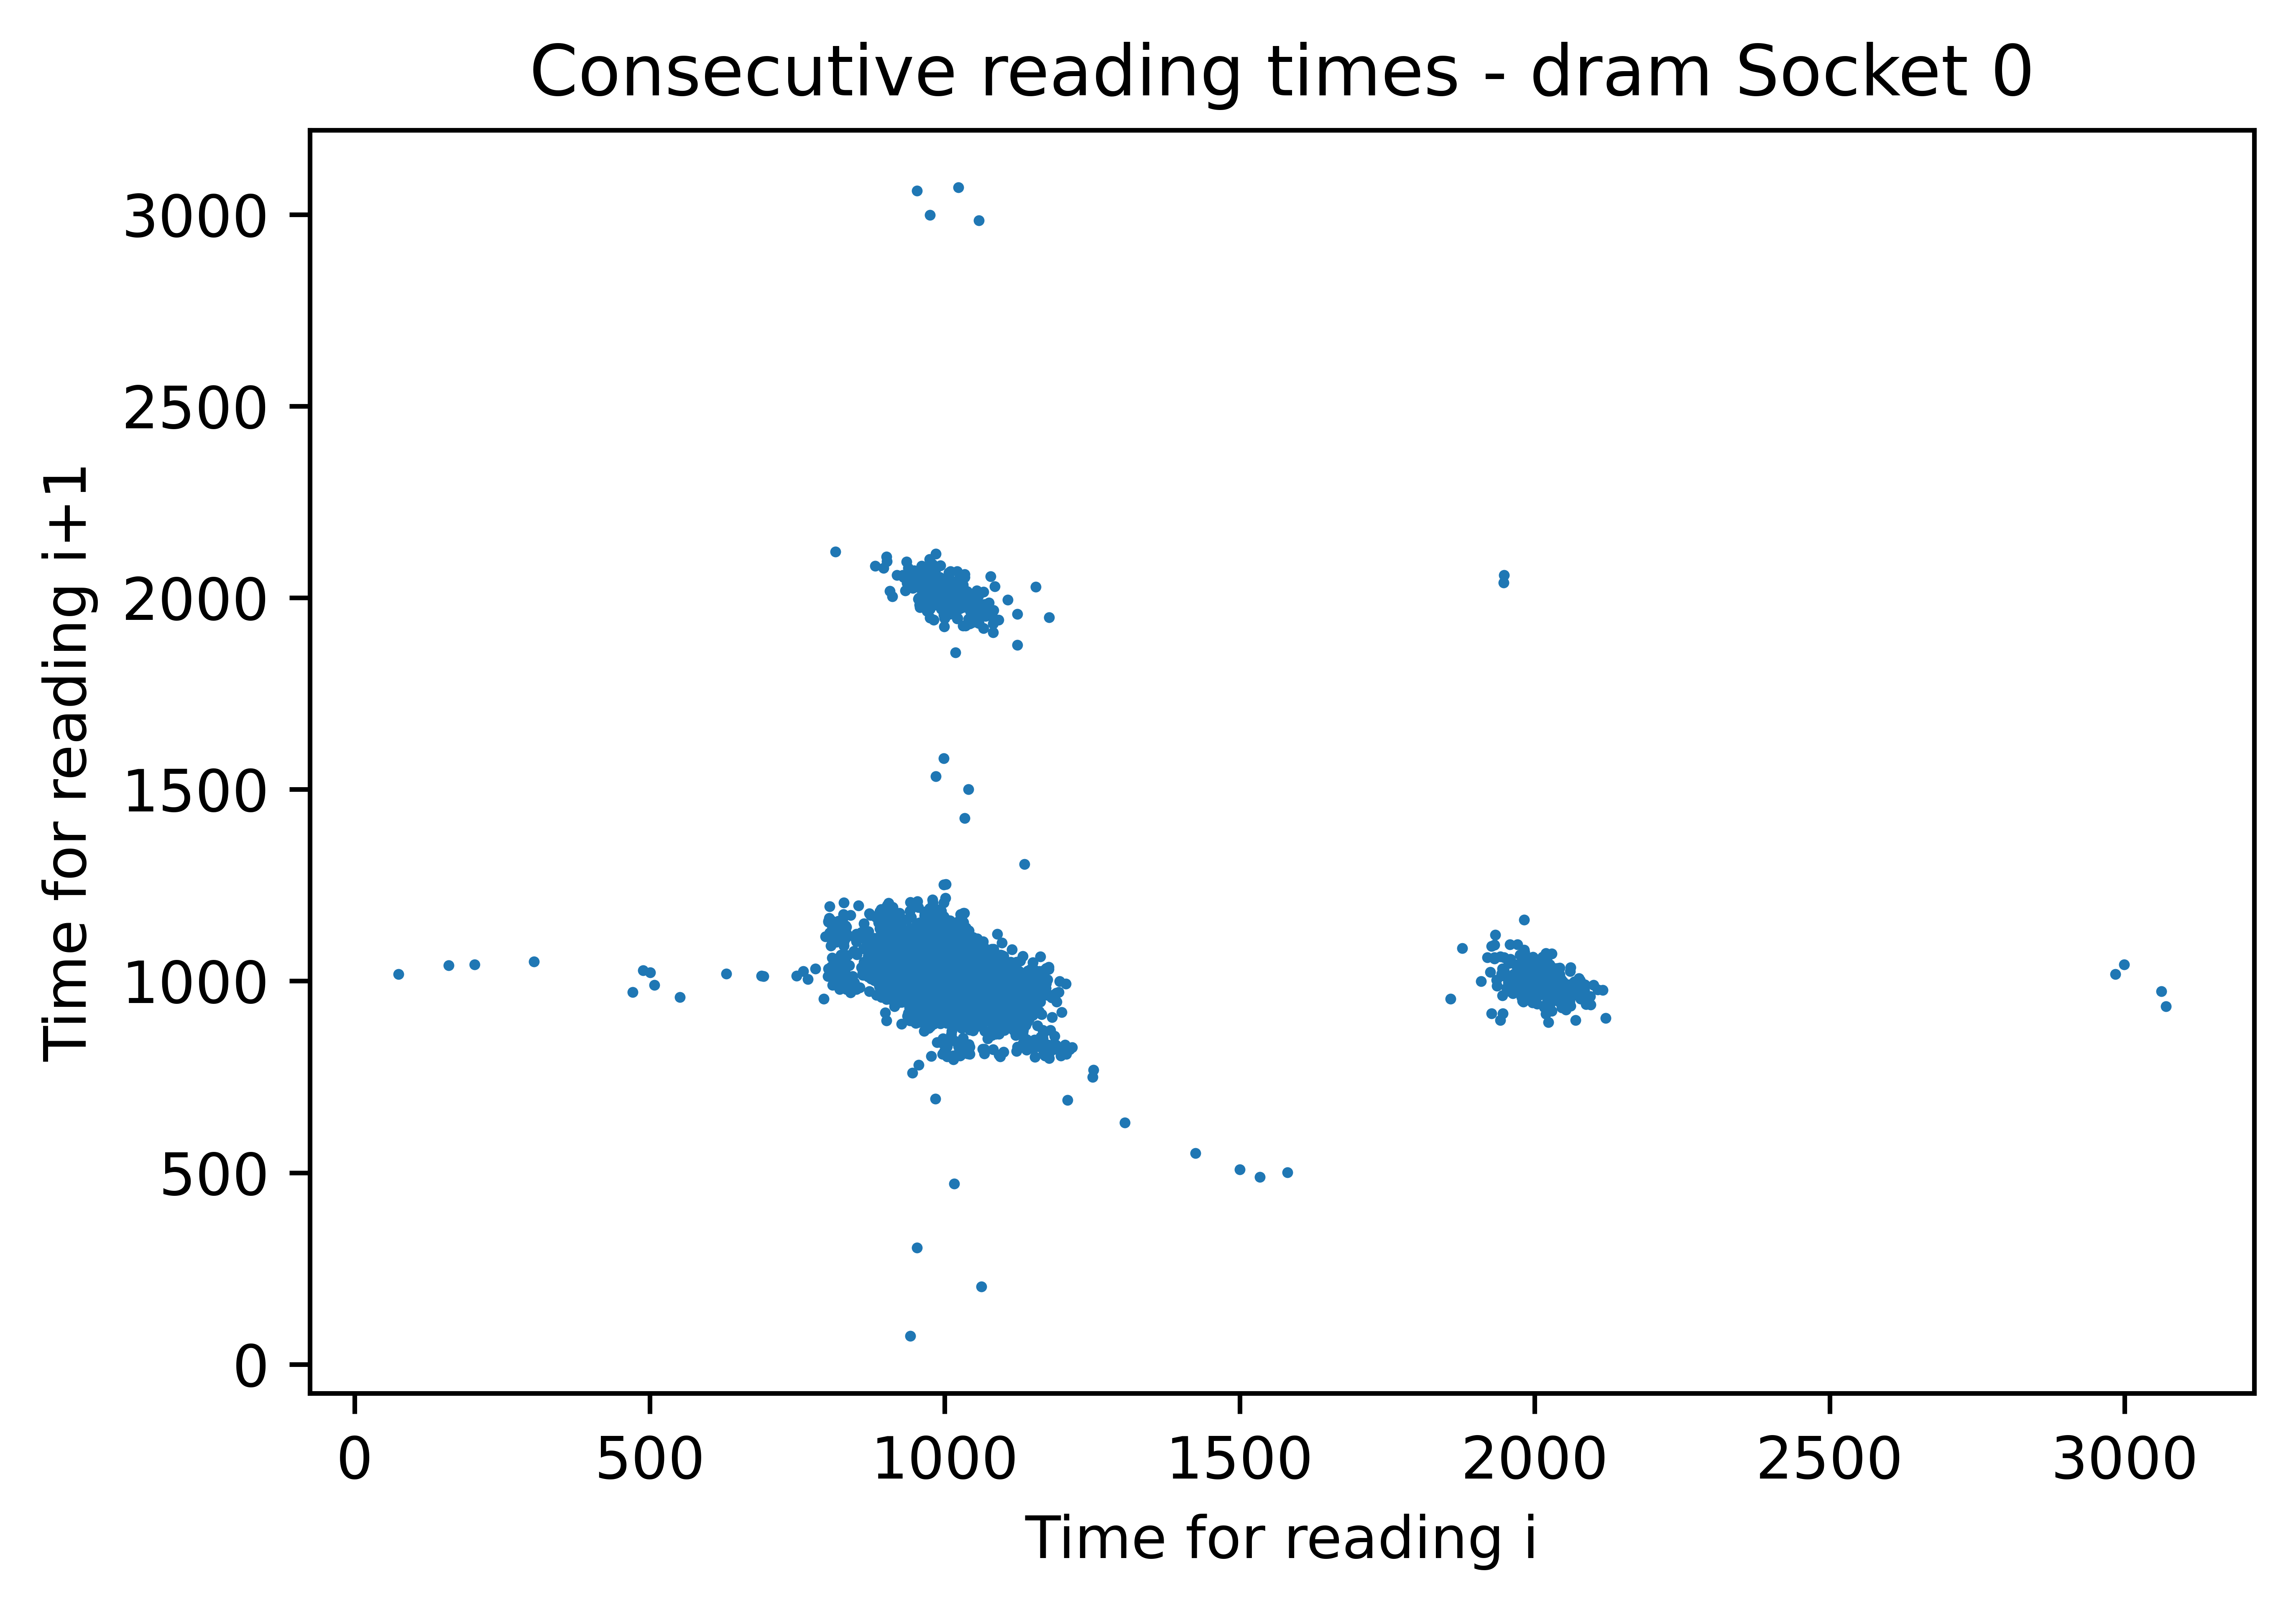
\includegraphics[width=10cm,height=10cm,keepaspectratio]{jmh/msr-update-rate/dram_Socket_0-i_n-v-i_n1.png}
    \caption{How long it takes for the PKG\_socket2 MSR to update (microseconds)}
    \label{fig:PKG-rapl-counter}
\end{figure}

\begin{figure}[H]
    \centering
    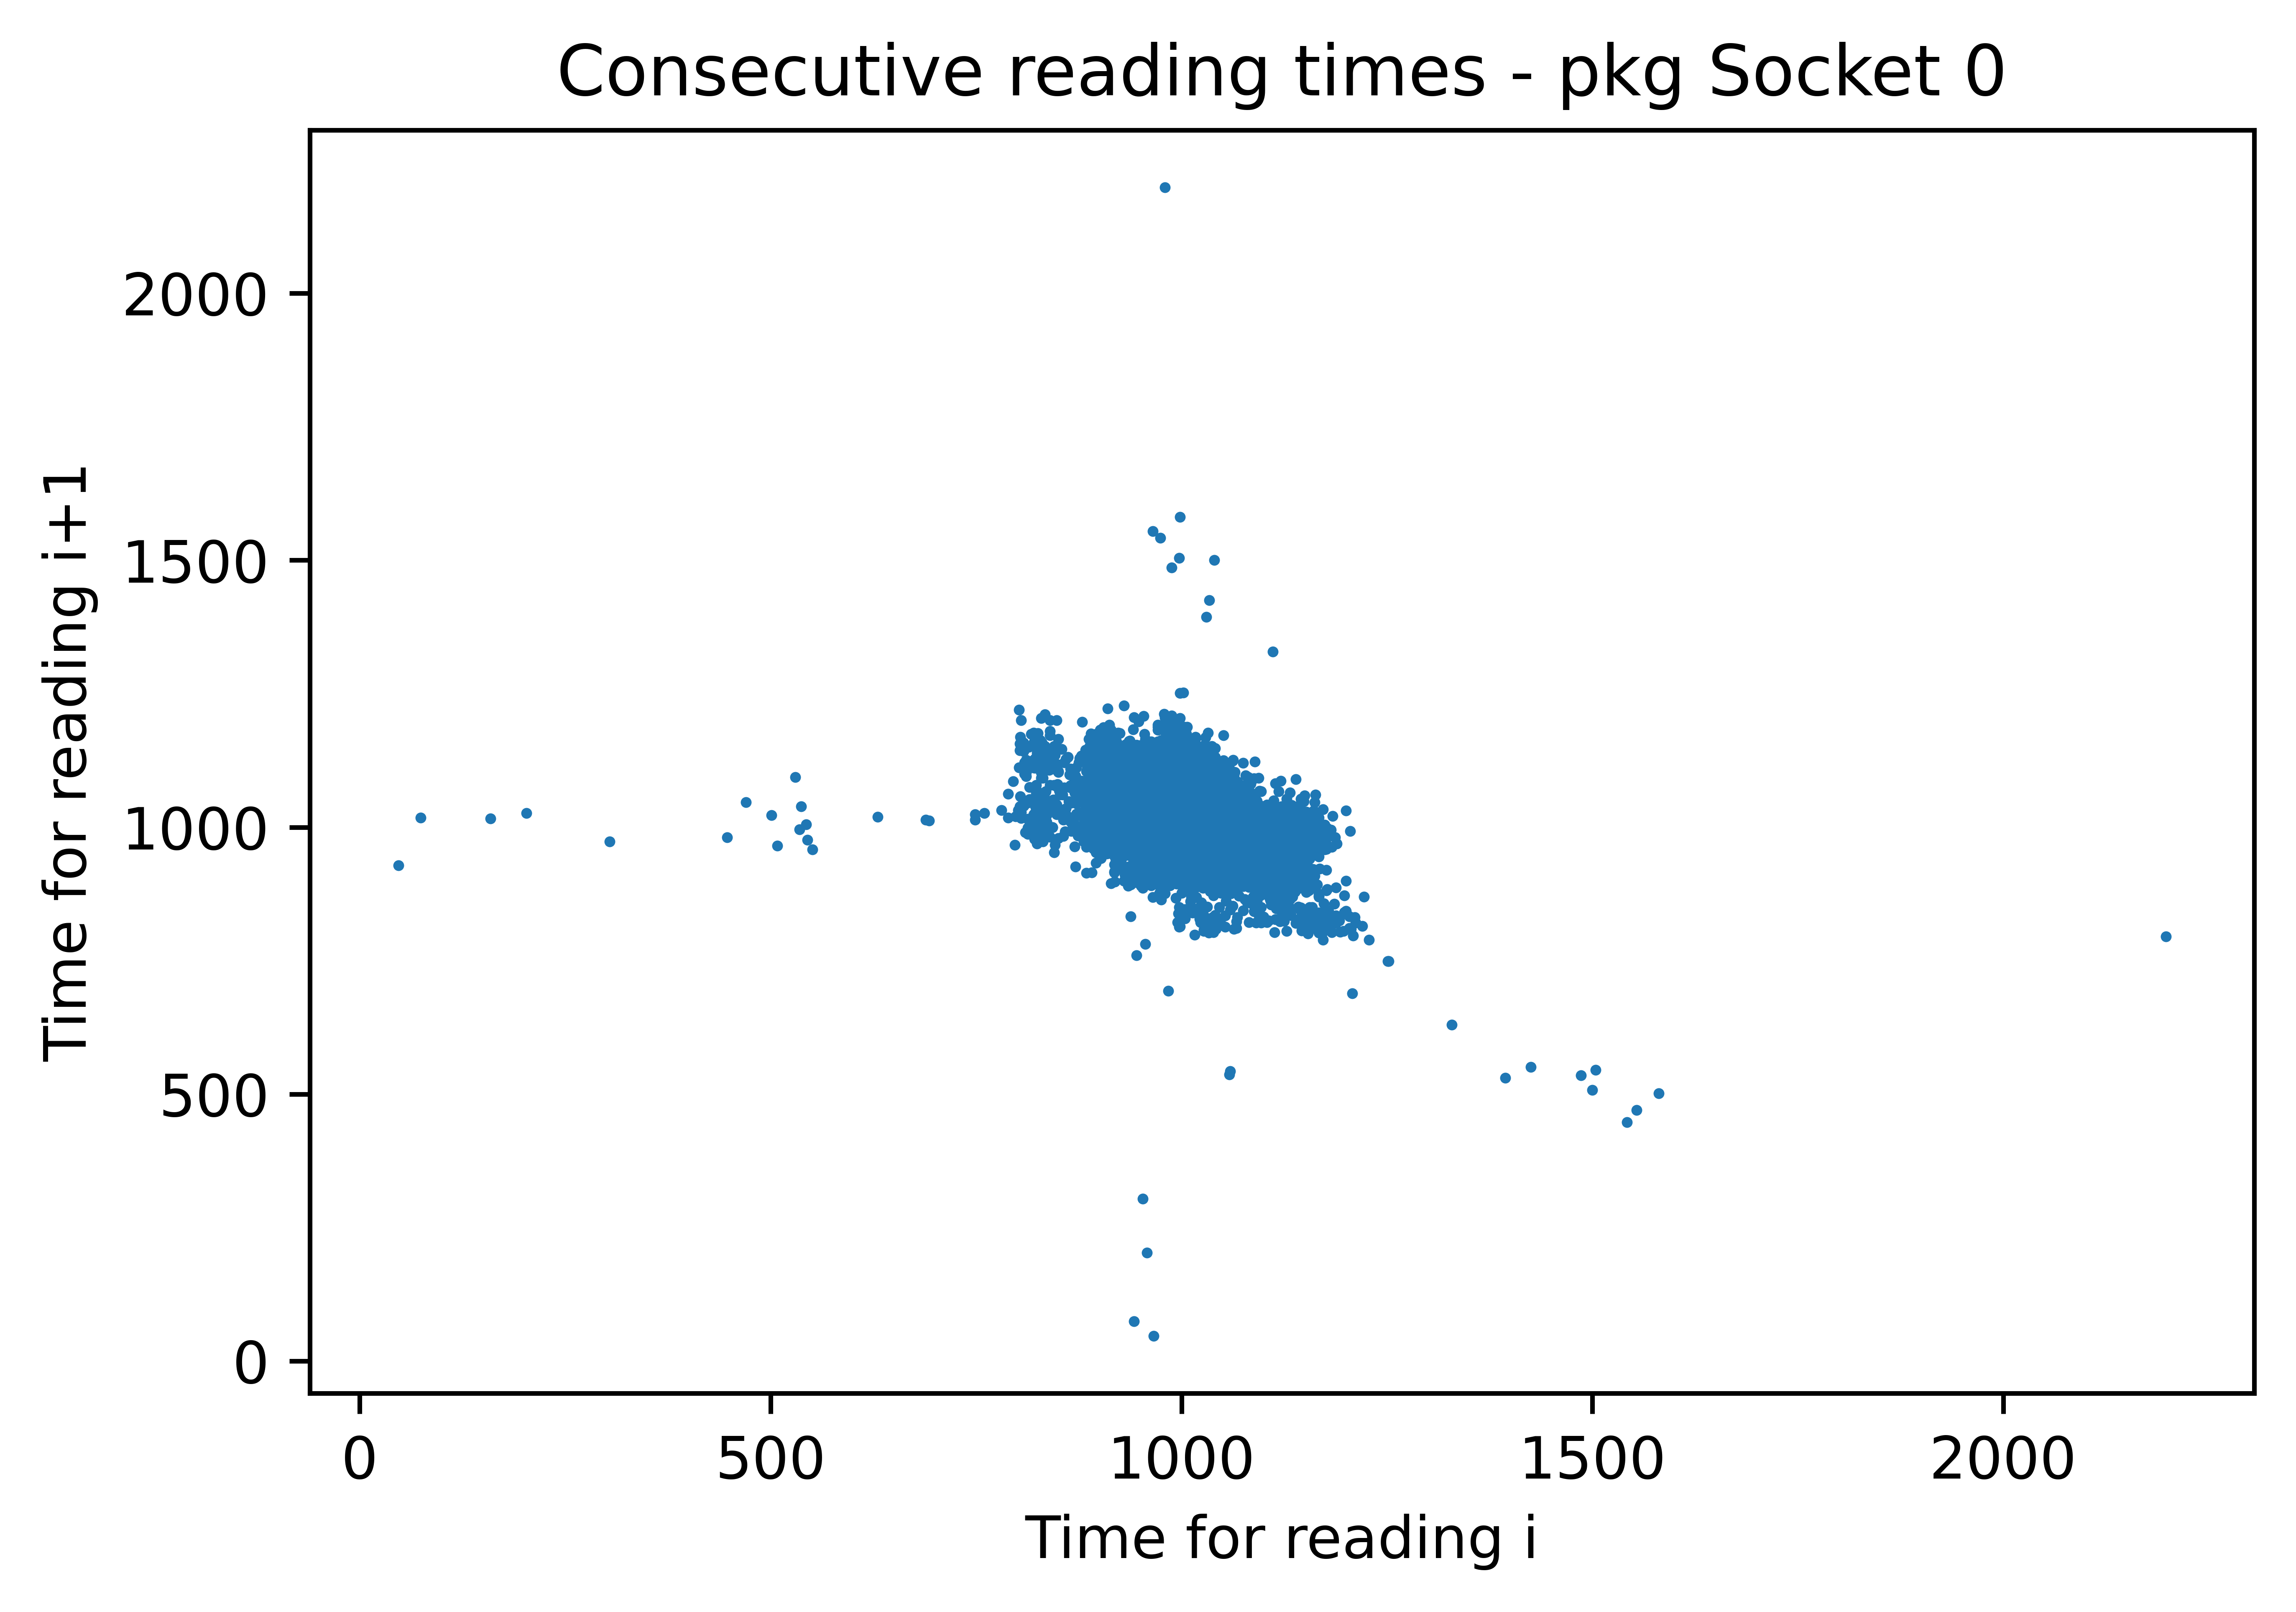
\includegraphics[width=10cm,height=10cm,keepaspectratio]{jmh/msr-update-rate/pkg_Socket_0-i_n-v-i_n1.png}
    \caption{How long it takes for the PKG\_socket2 MSR to update (microseconds)}
    \label{fig:PKG-rapl-counter}
\end{figure}

\begin{figure}[H]
    \centering
    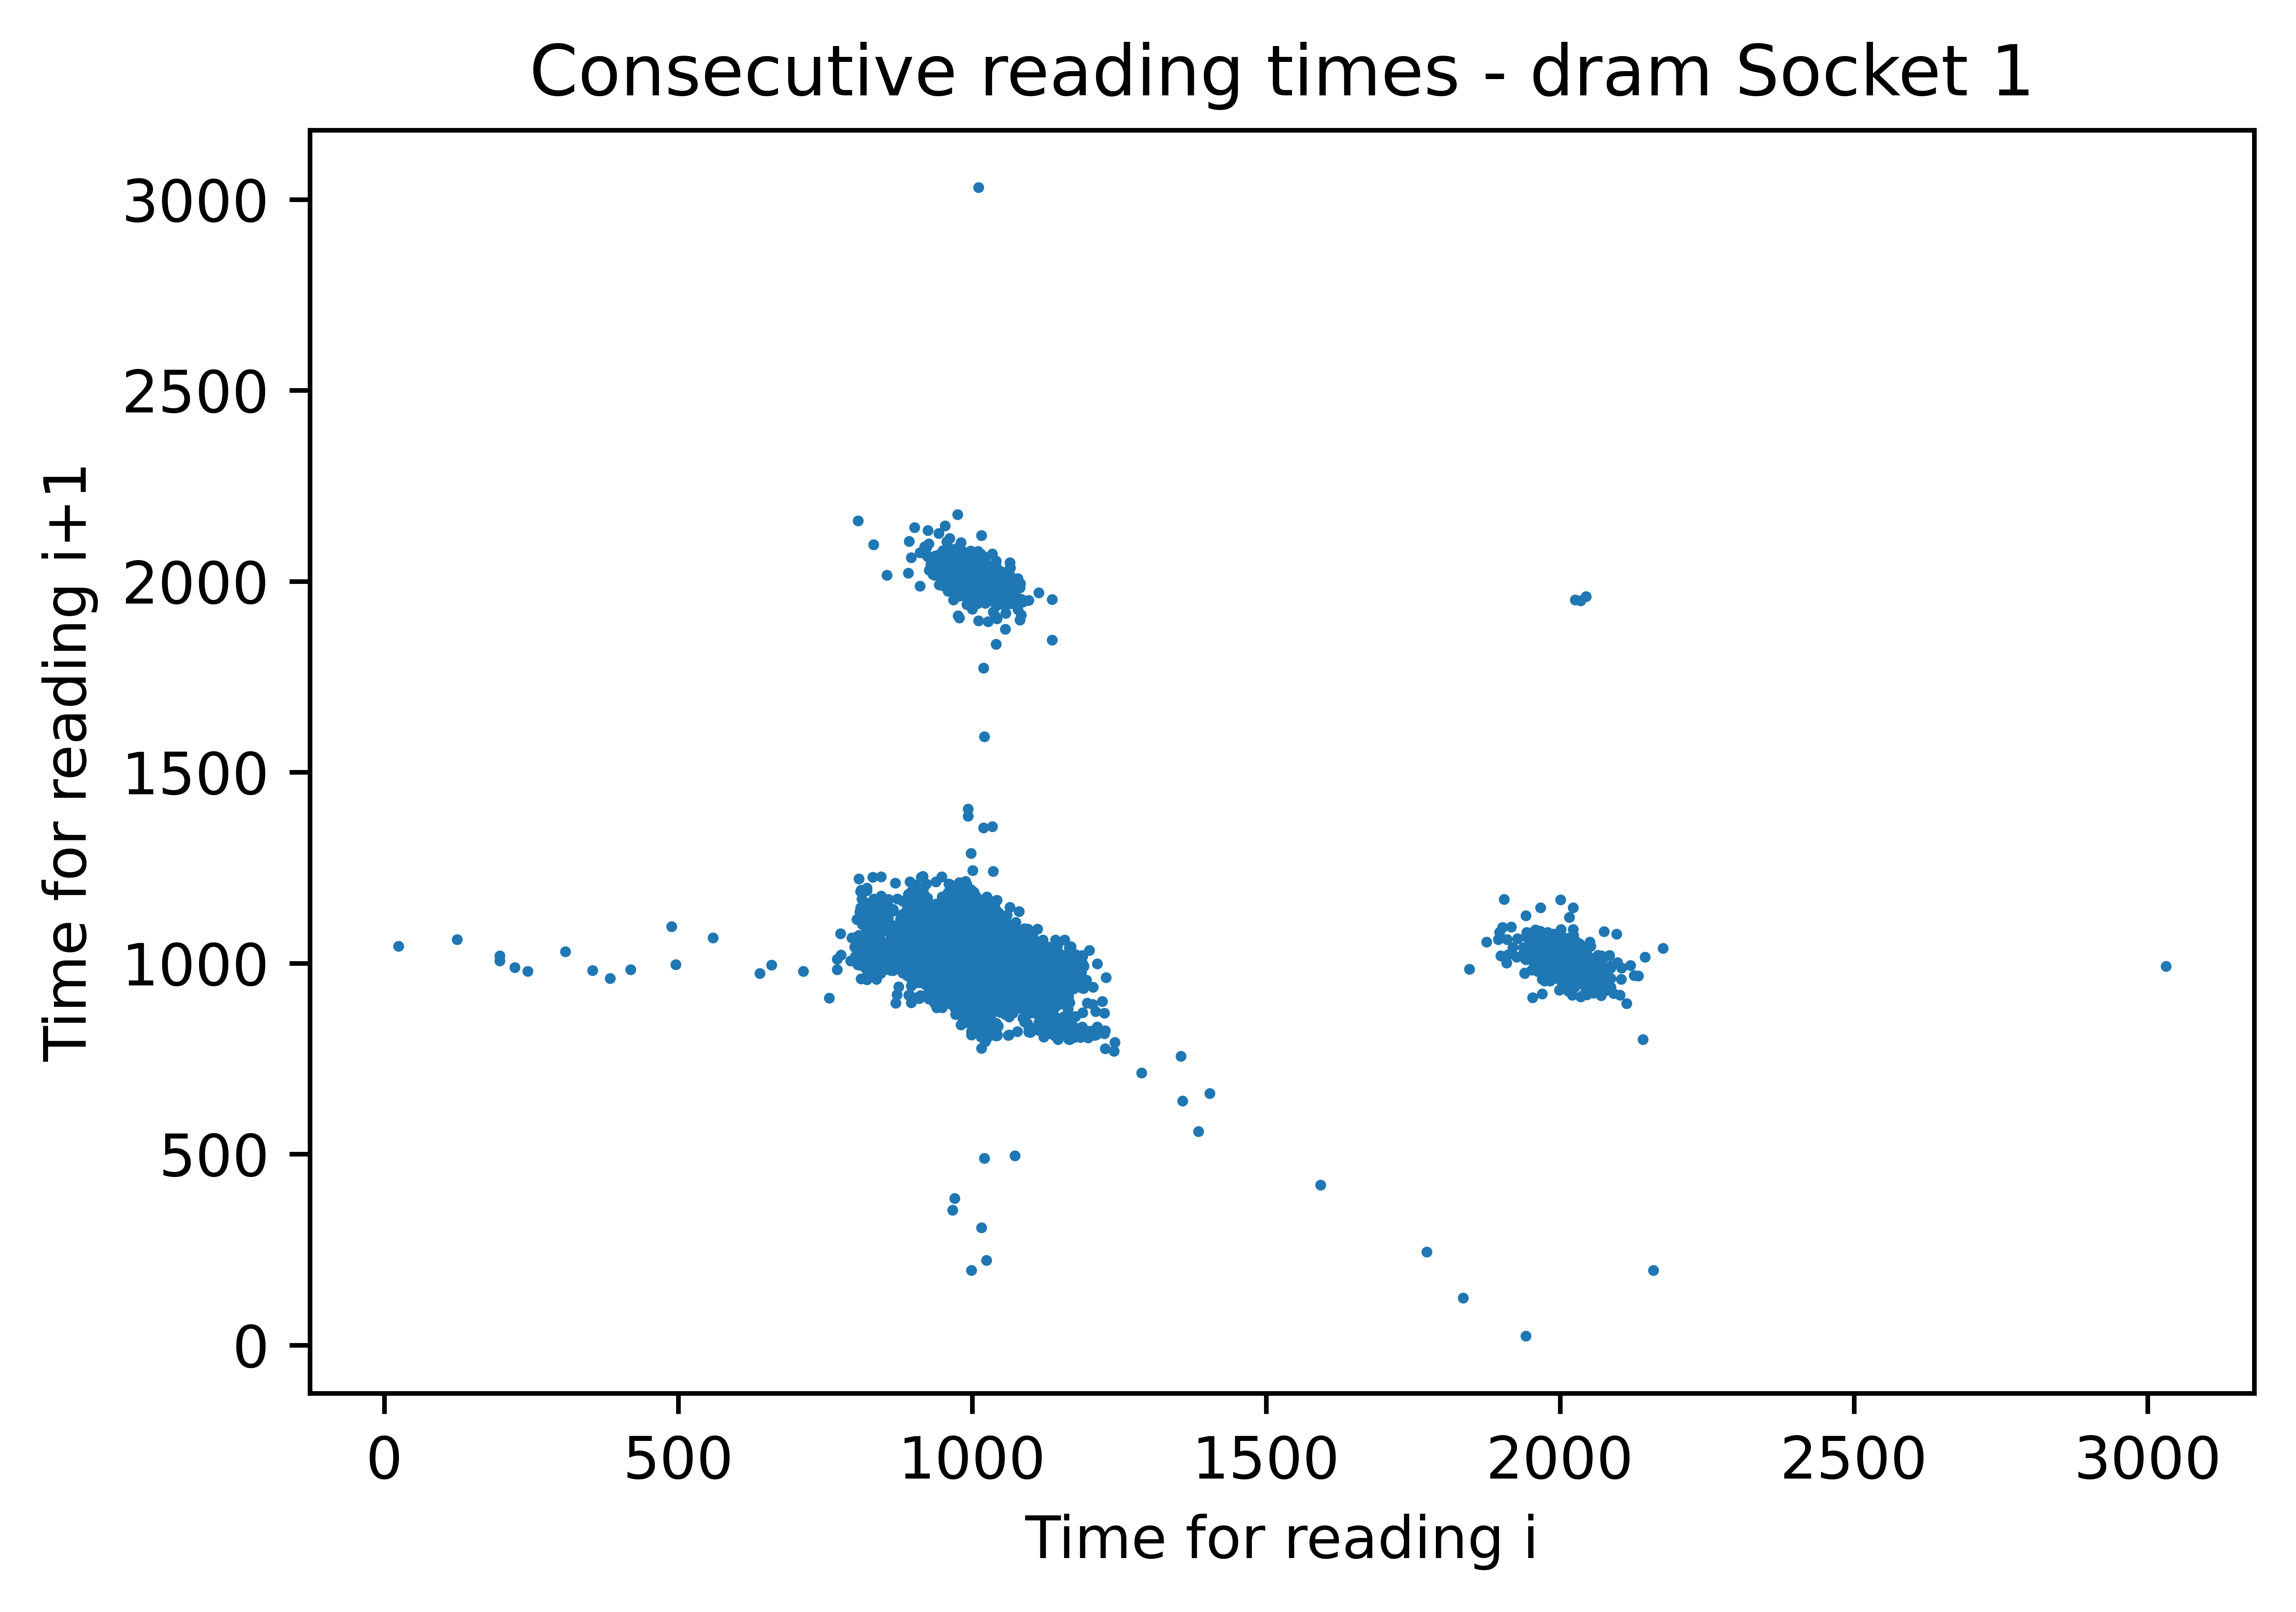
\includegraphics[width=10cm,height=10cm,keepaspectratio]{jmh/msr-update-rate/dram_Socket_1-i_n-v-i_n1.png}
    \caption{How long it takes for the PKG\_socket2 MSR to update (microseconds)}
    \label{fig:PKG-rapl-counter}
\end{figure}

\begin{figure}[H]
    \centering
    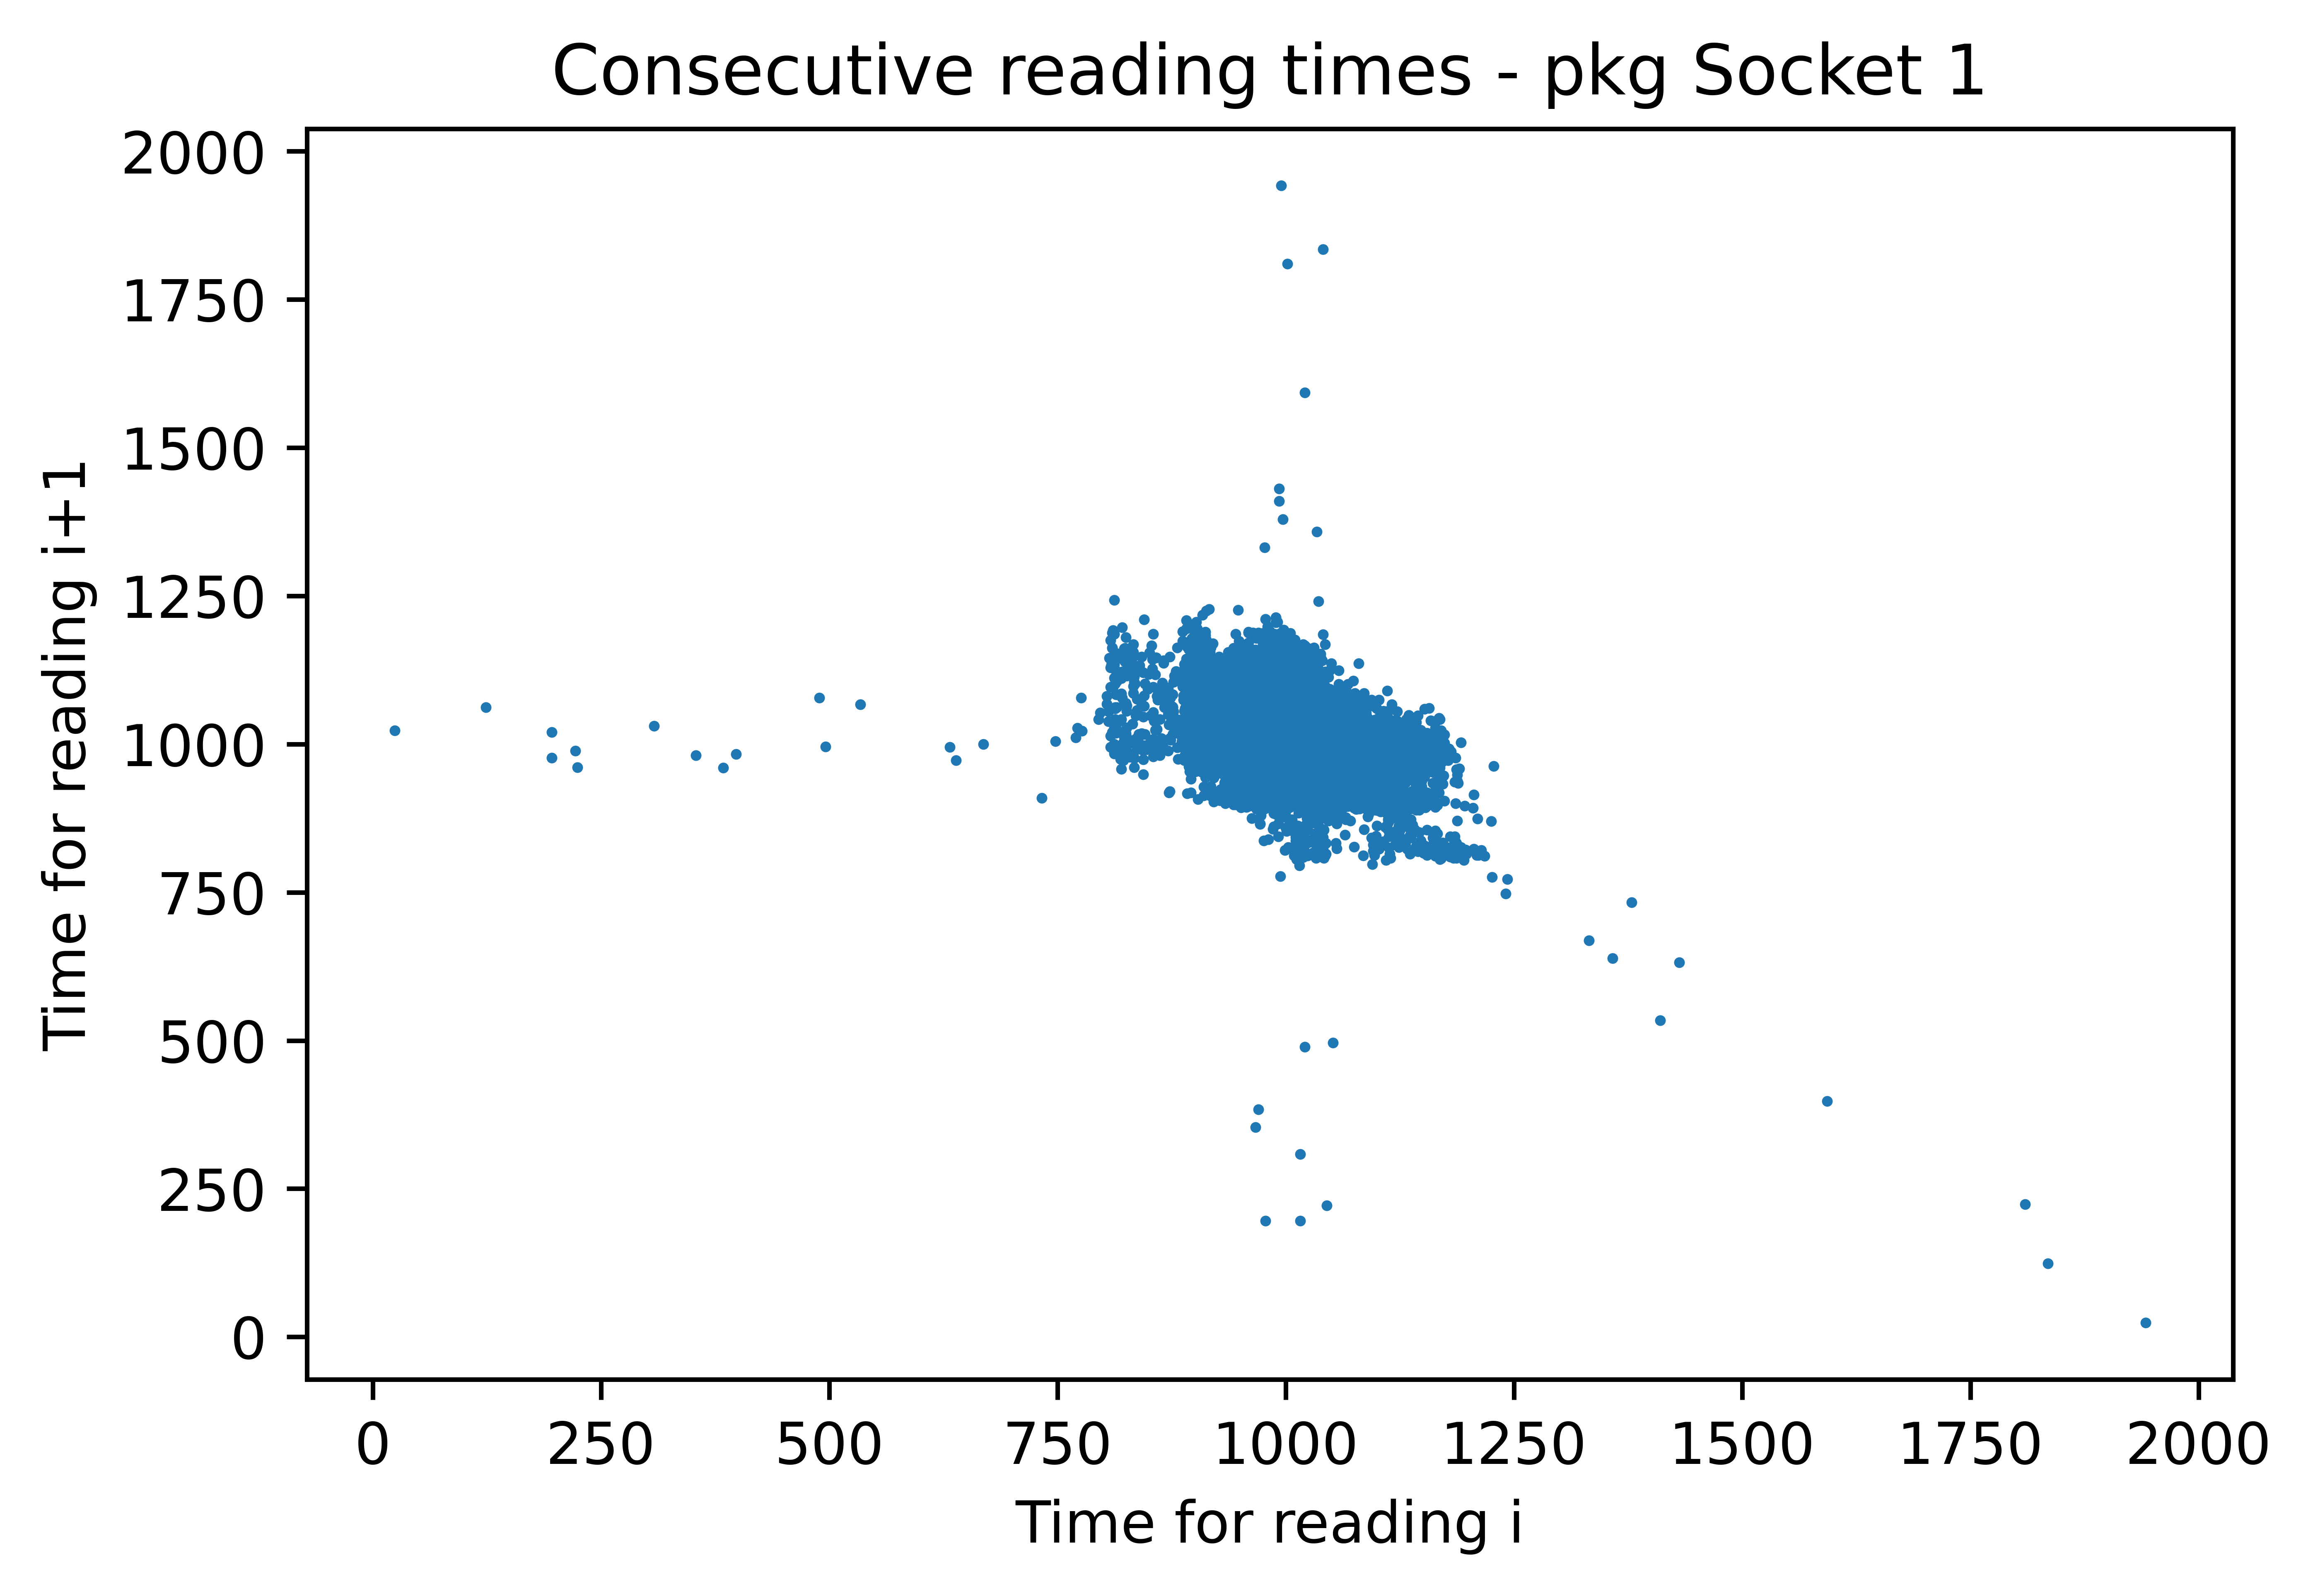
\includegraphics[width=10cm,height=10cm,keepaspectratio]{jmh/msr-update-rate/pkg_Socket_1-i_n-v-i_n1.png}
    \caption{How long it takes for the PKG\_socket2 MSR to update (microseconds)}
    \label{fig:PKG-rapl-counter}
\end{figure}

\begin{figure}[H]
    \centering
    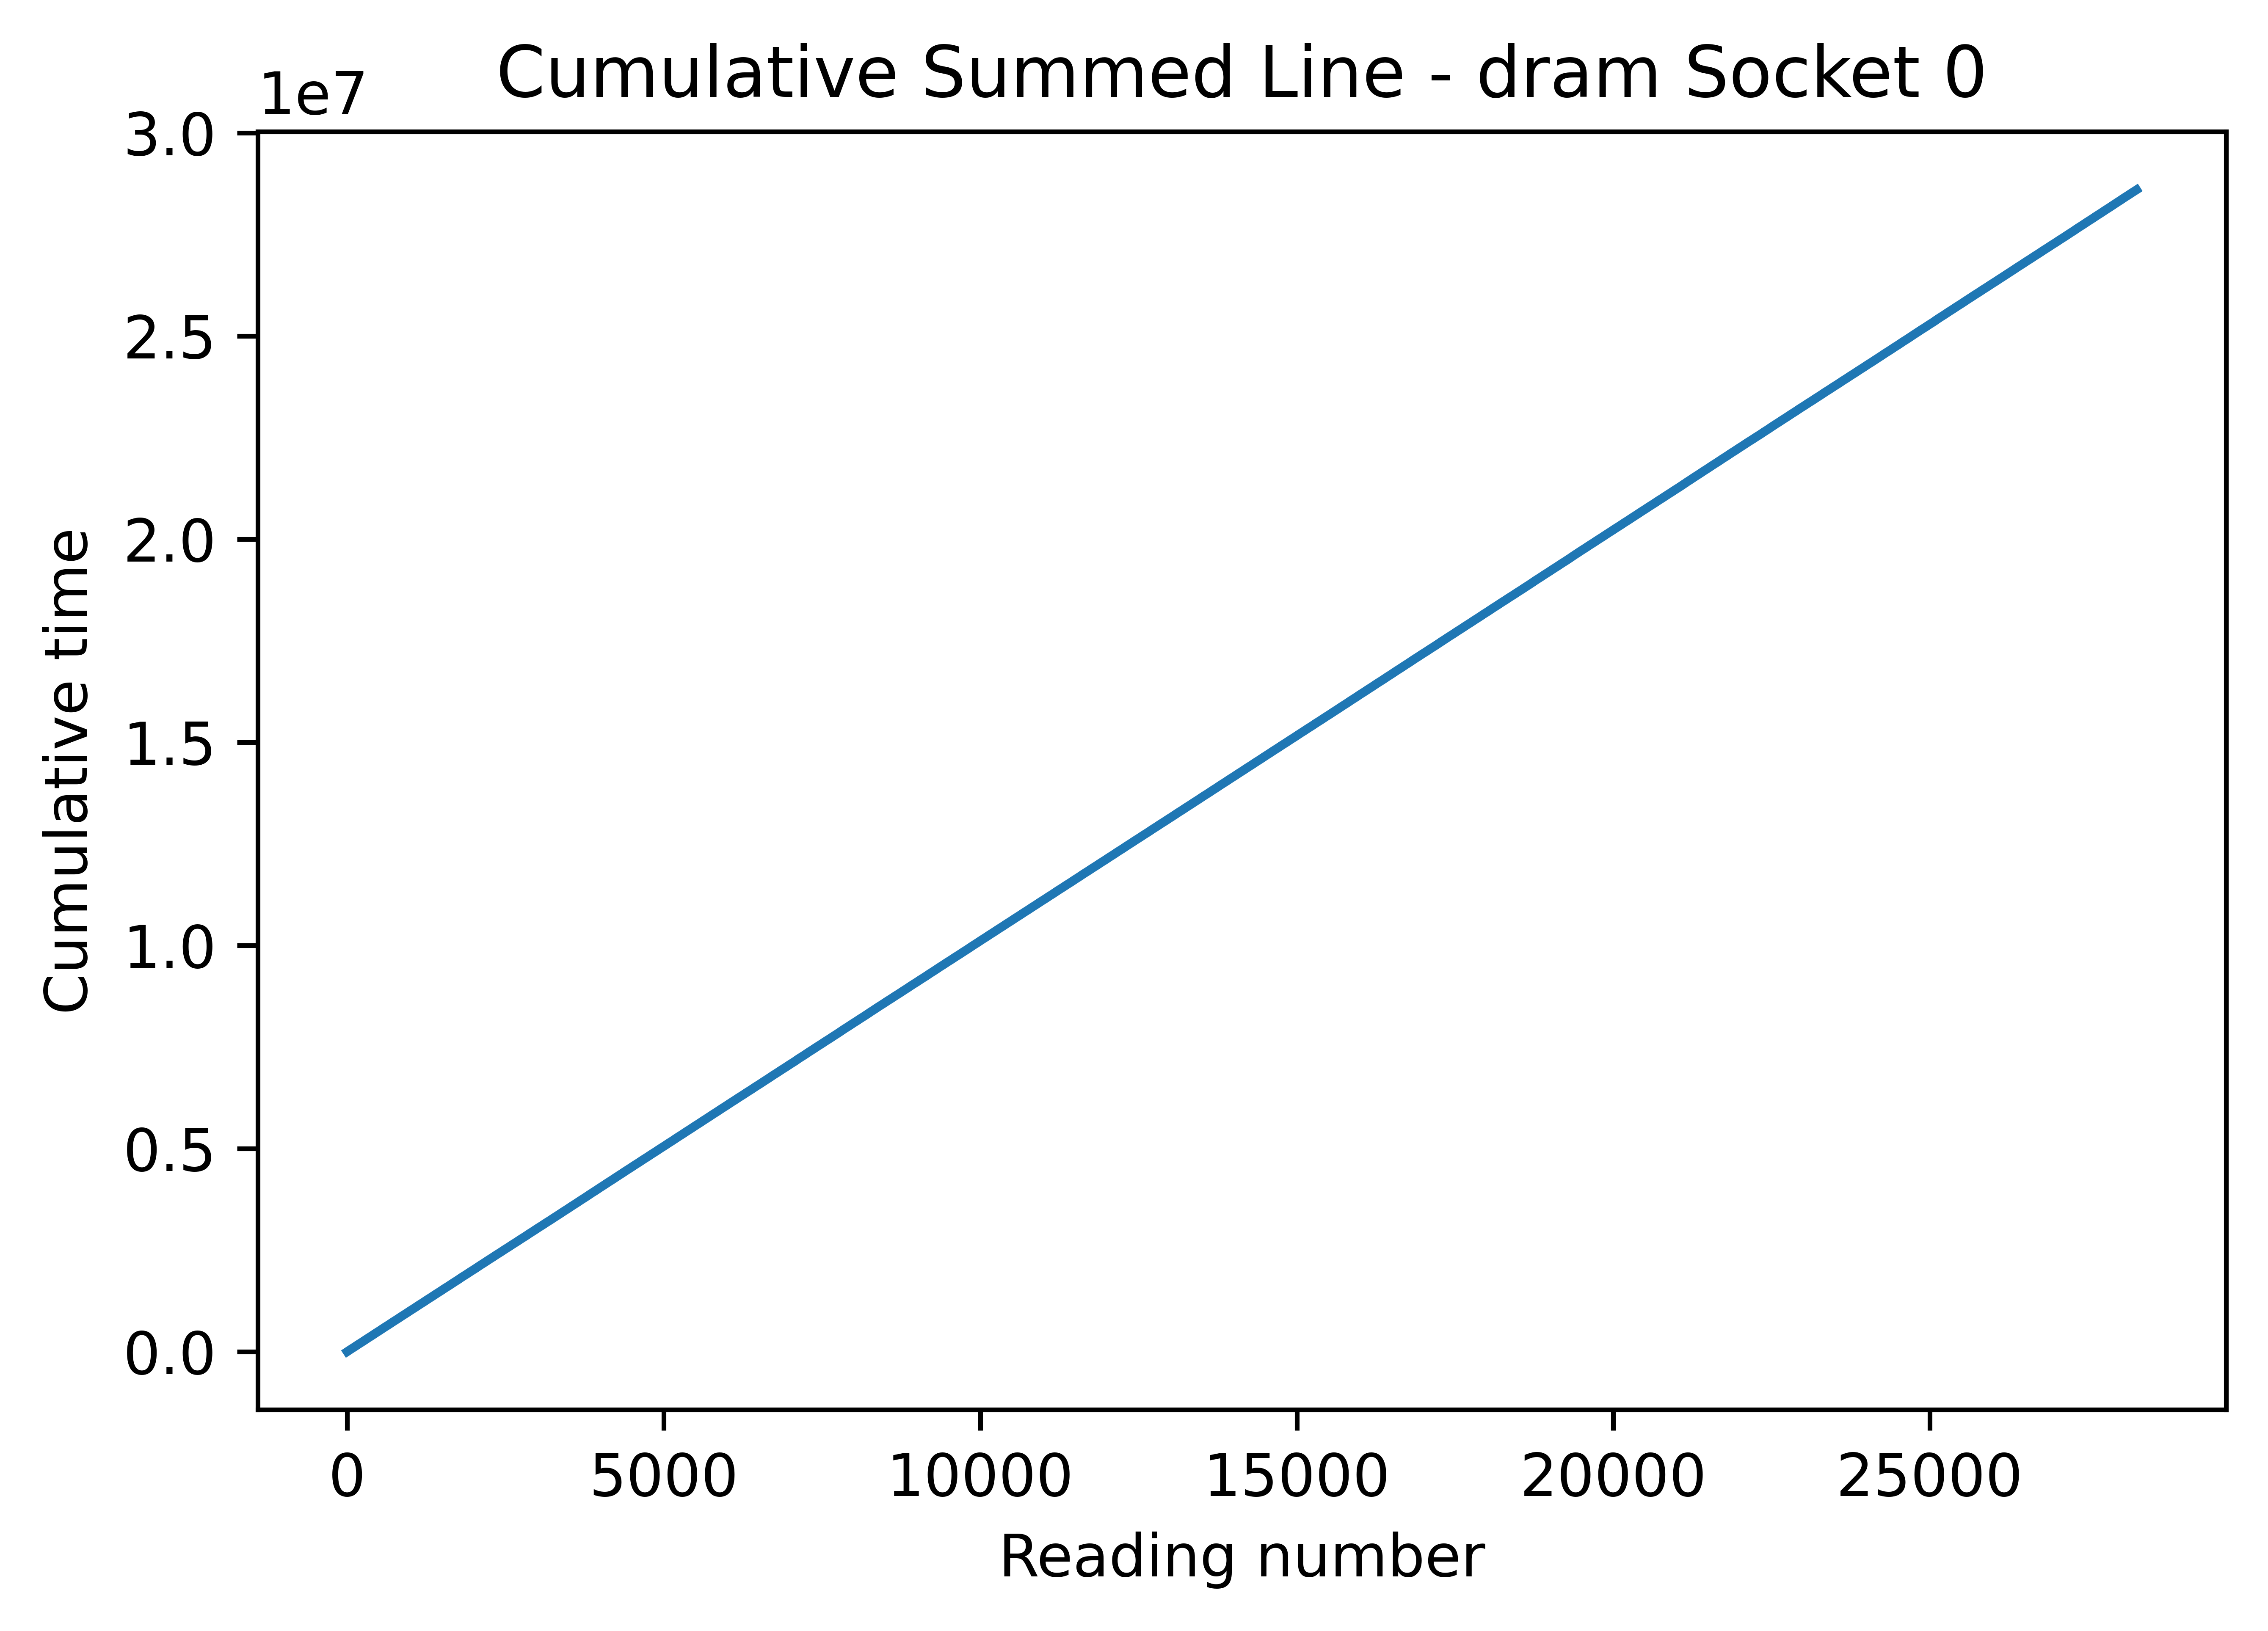
\includegraphics[width=10cm,height=10cm,keepaspectratio]{jmh/msr-update-rate/dram_Socket_0-cumulative-summed.png}
    \caption{How long it takes for the PKG\_socket2 MSR to update (microseconds)}
    \label{fig:PKG-rapl-counter}
\end{figure}

\begin{figure}[H]
    \centering
    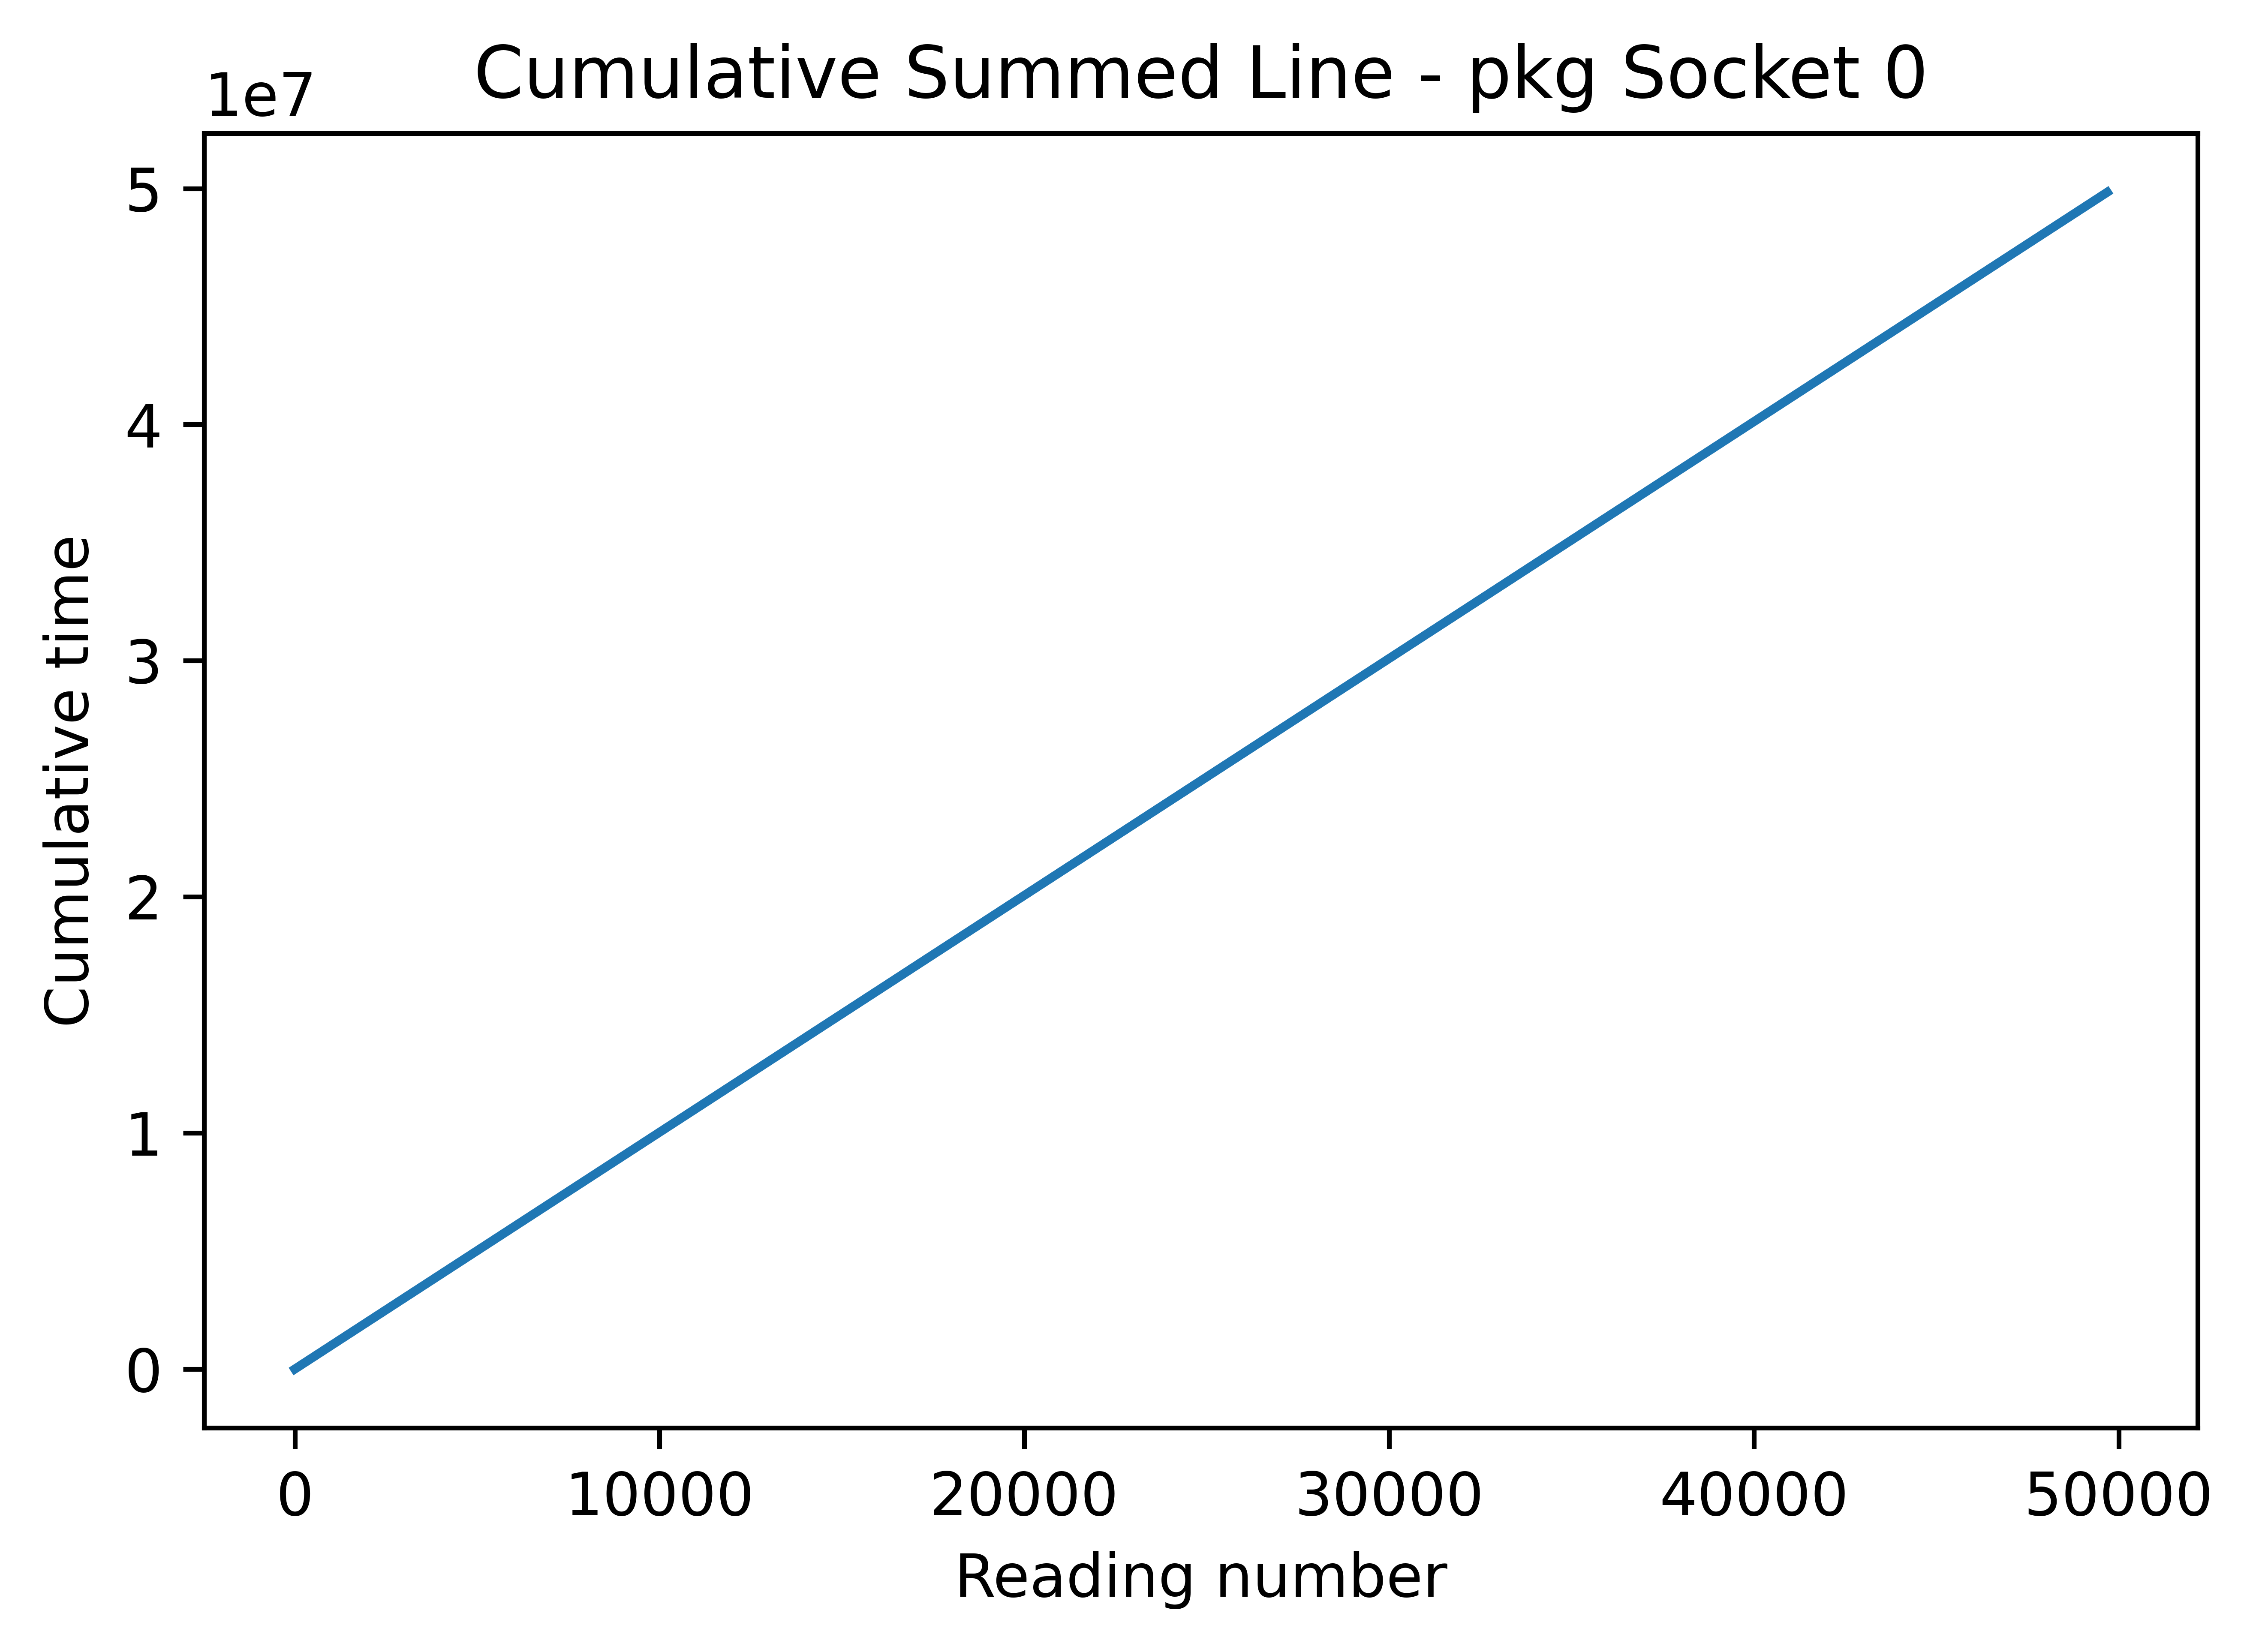
\includegraphics[width=10cm,height=10cm,keepaspectratio]{jmh/msr-update-rate/pkg_Socket_0-cumulative-summed.png}
    \caption{How long it takes for the PKG\_socket2 MSR to update (microseconds)}
    \label{fig:PKG-rapl-counter}
\end{figure}

\begin{figure}[H]
    \centering
    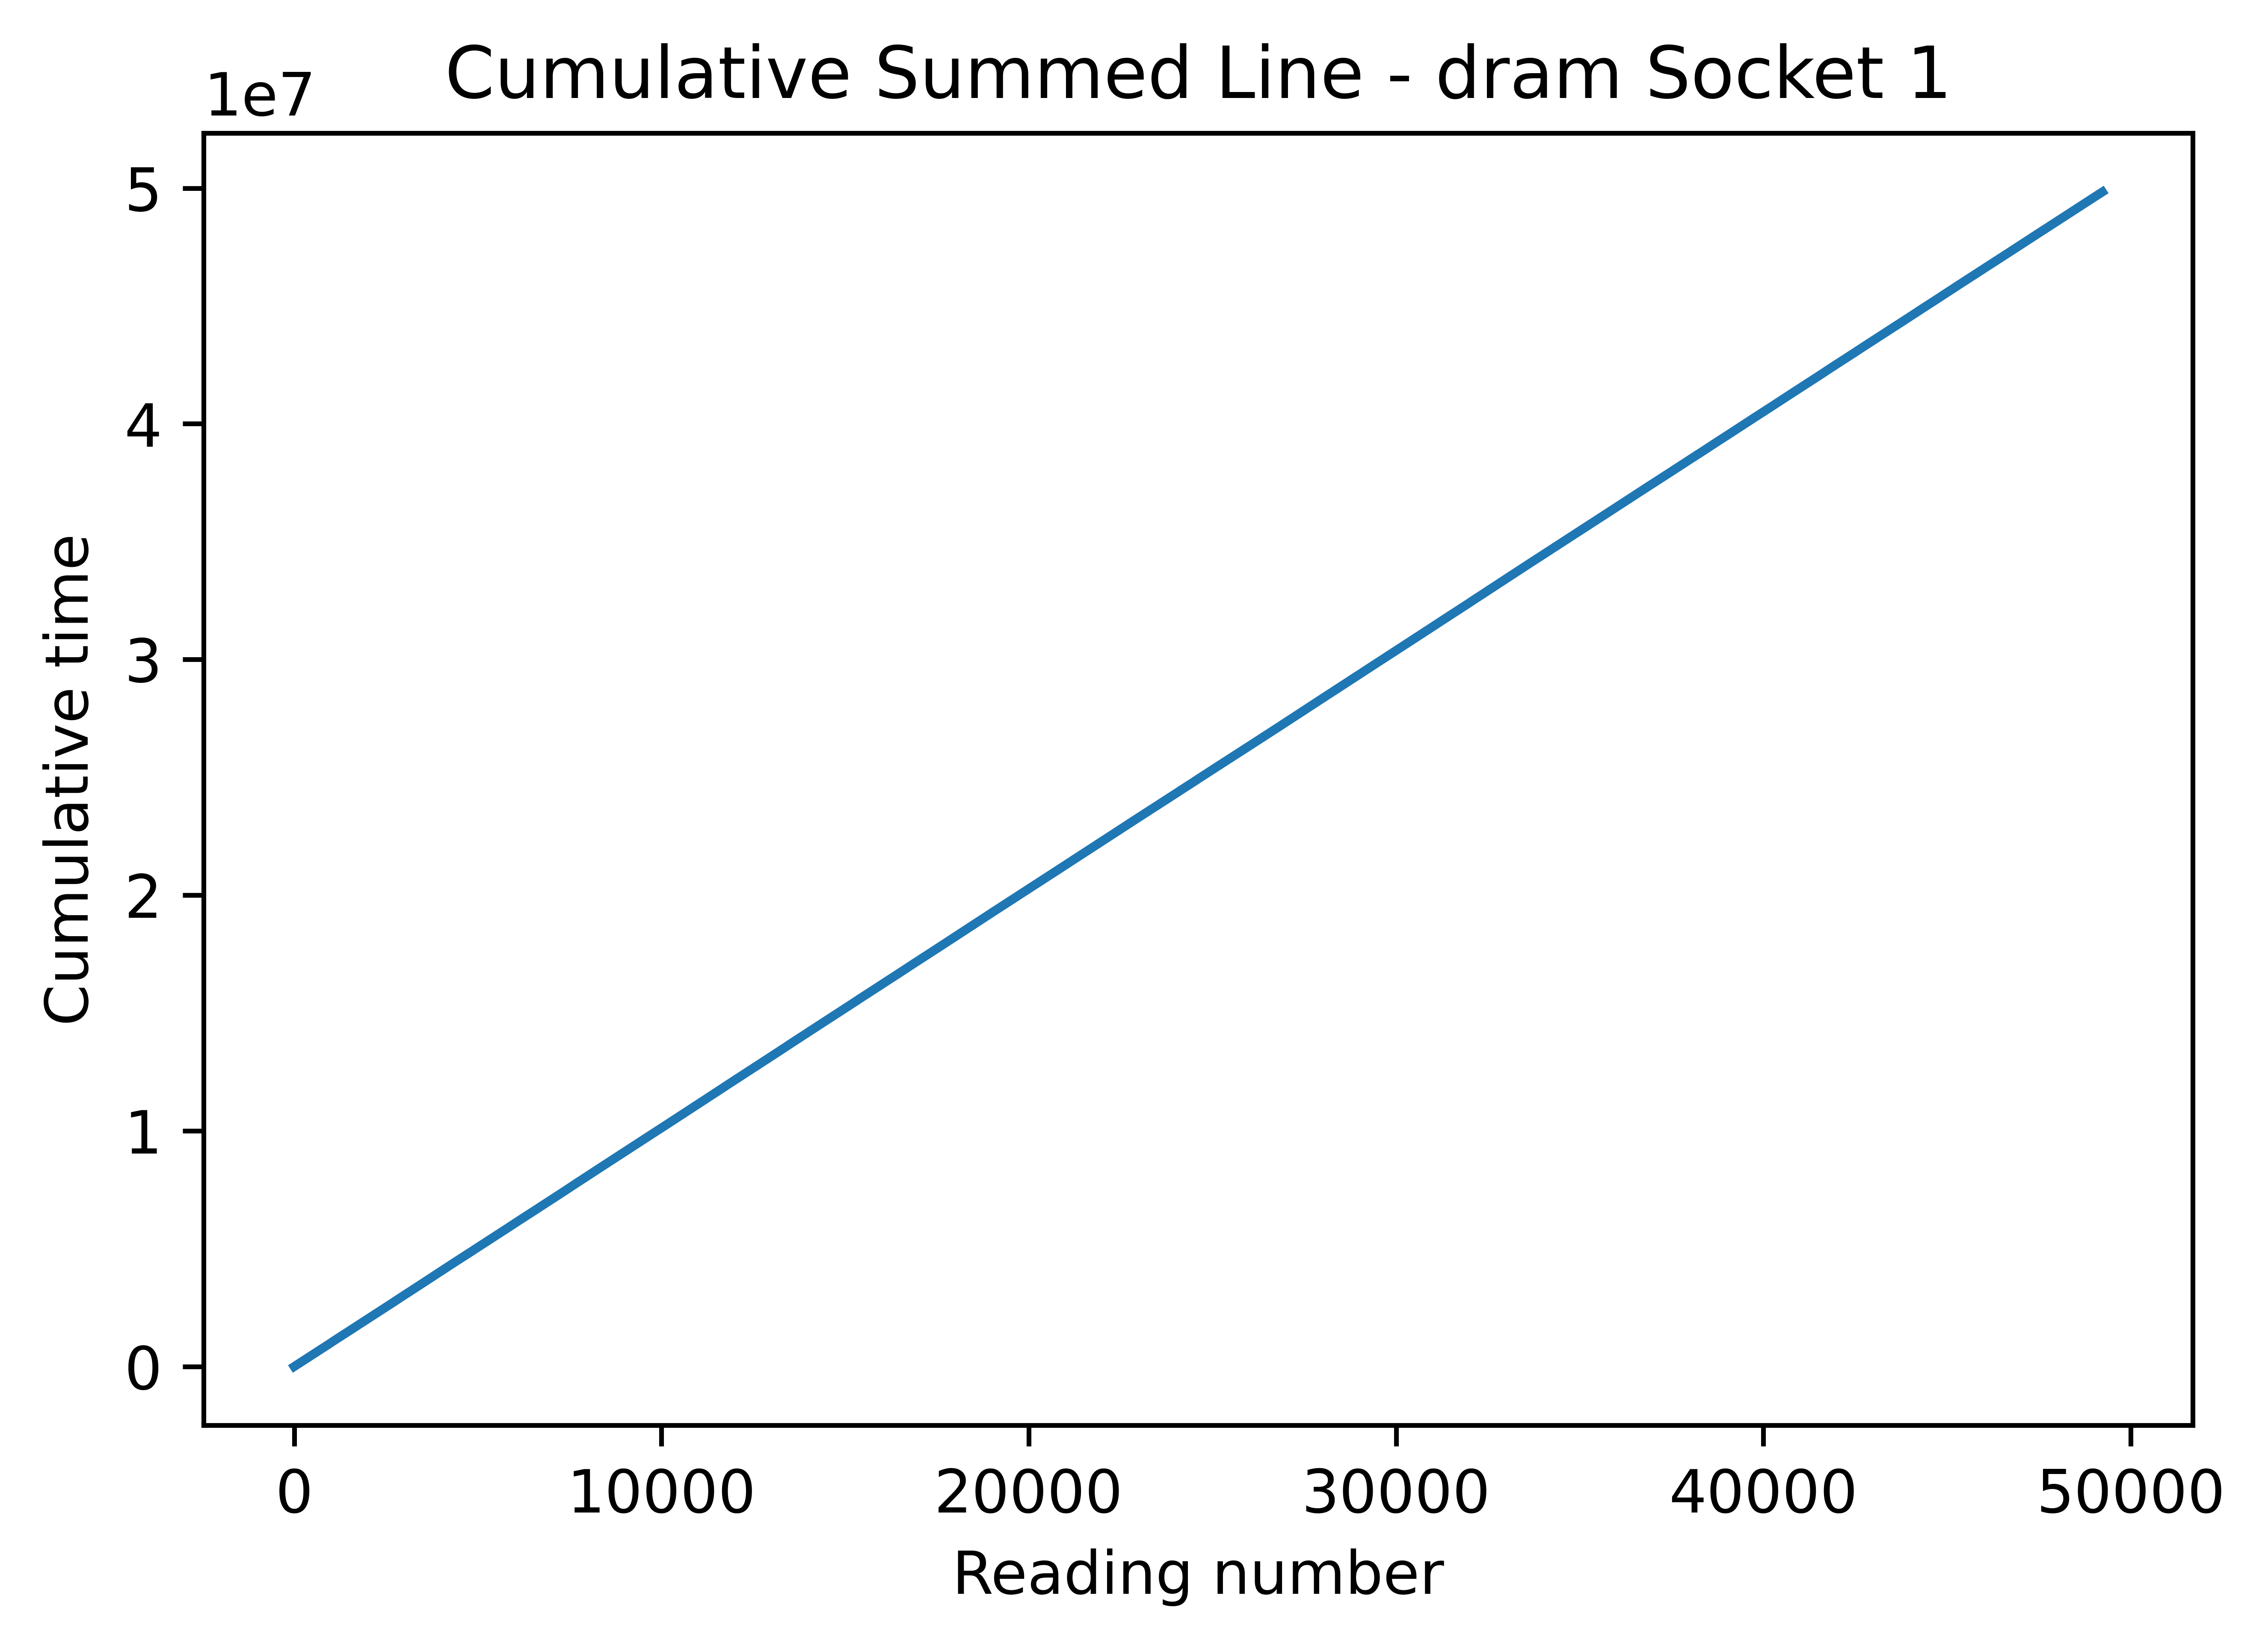
\includegraphics[width=10cm,height=10cm,keepaspectratio]{jmh/msr-update-rate/dram_Socket_1-cumulative-summed.png}
    \caption{How long it takes for the PKG\_socket2 MSR to update (microseconds)}
    \label{fig:PKG-rapl-counter}
\end{figure}

\begin{figure}[H]
    \centering
    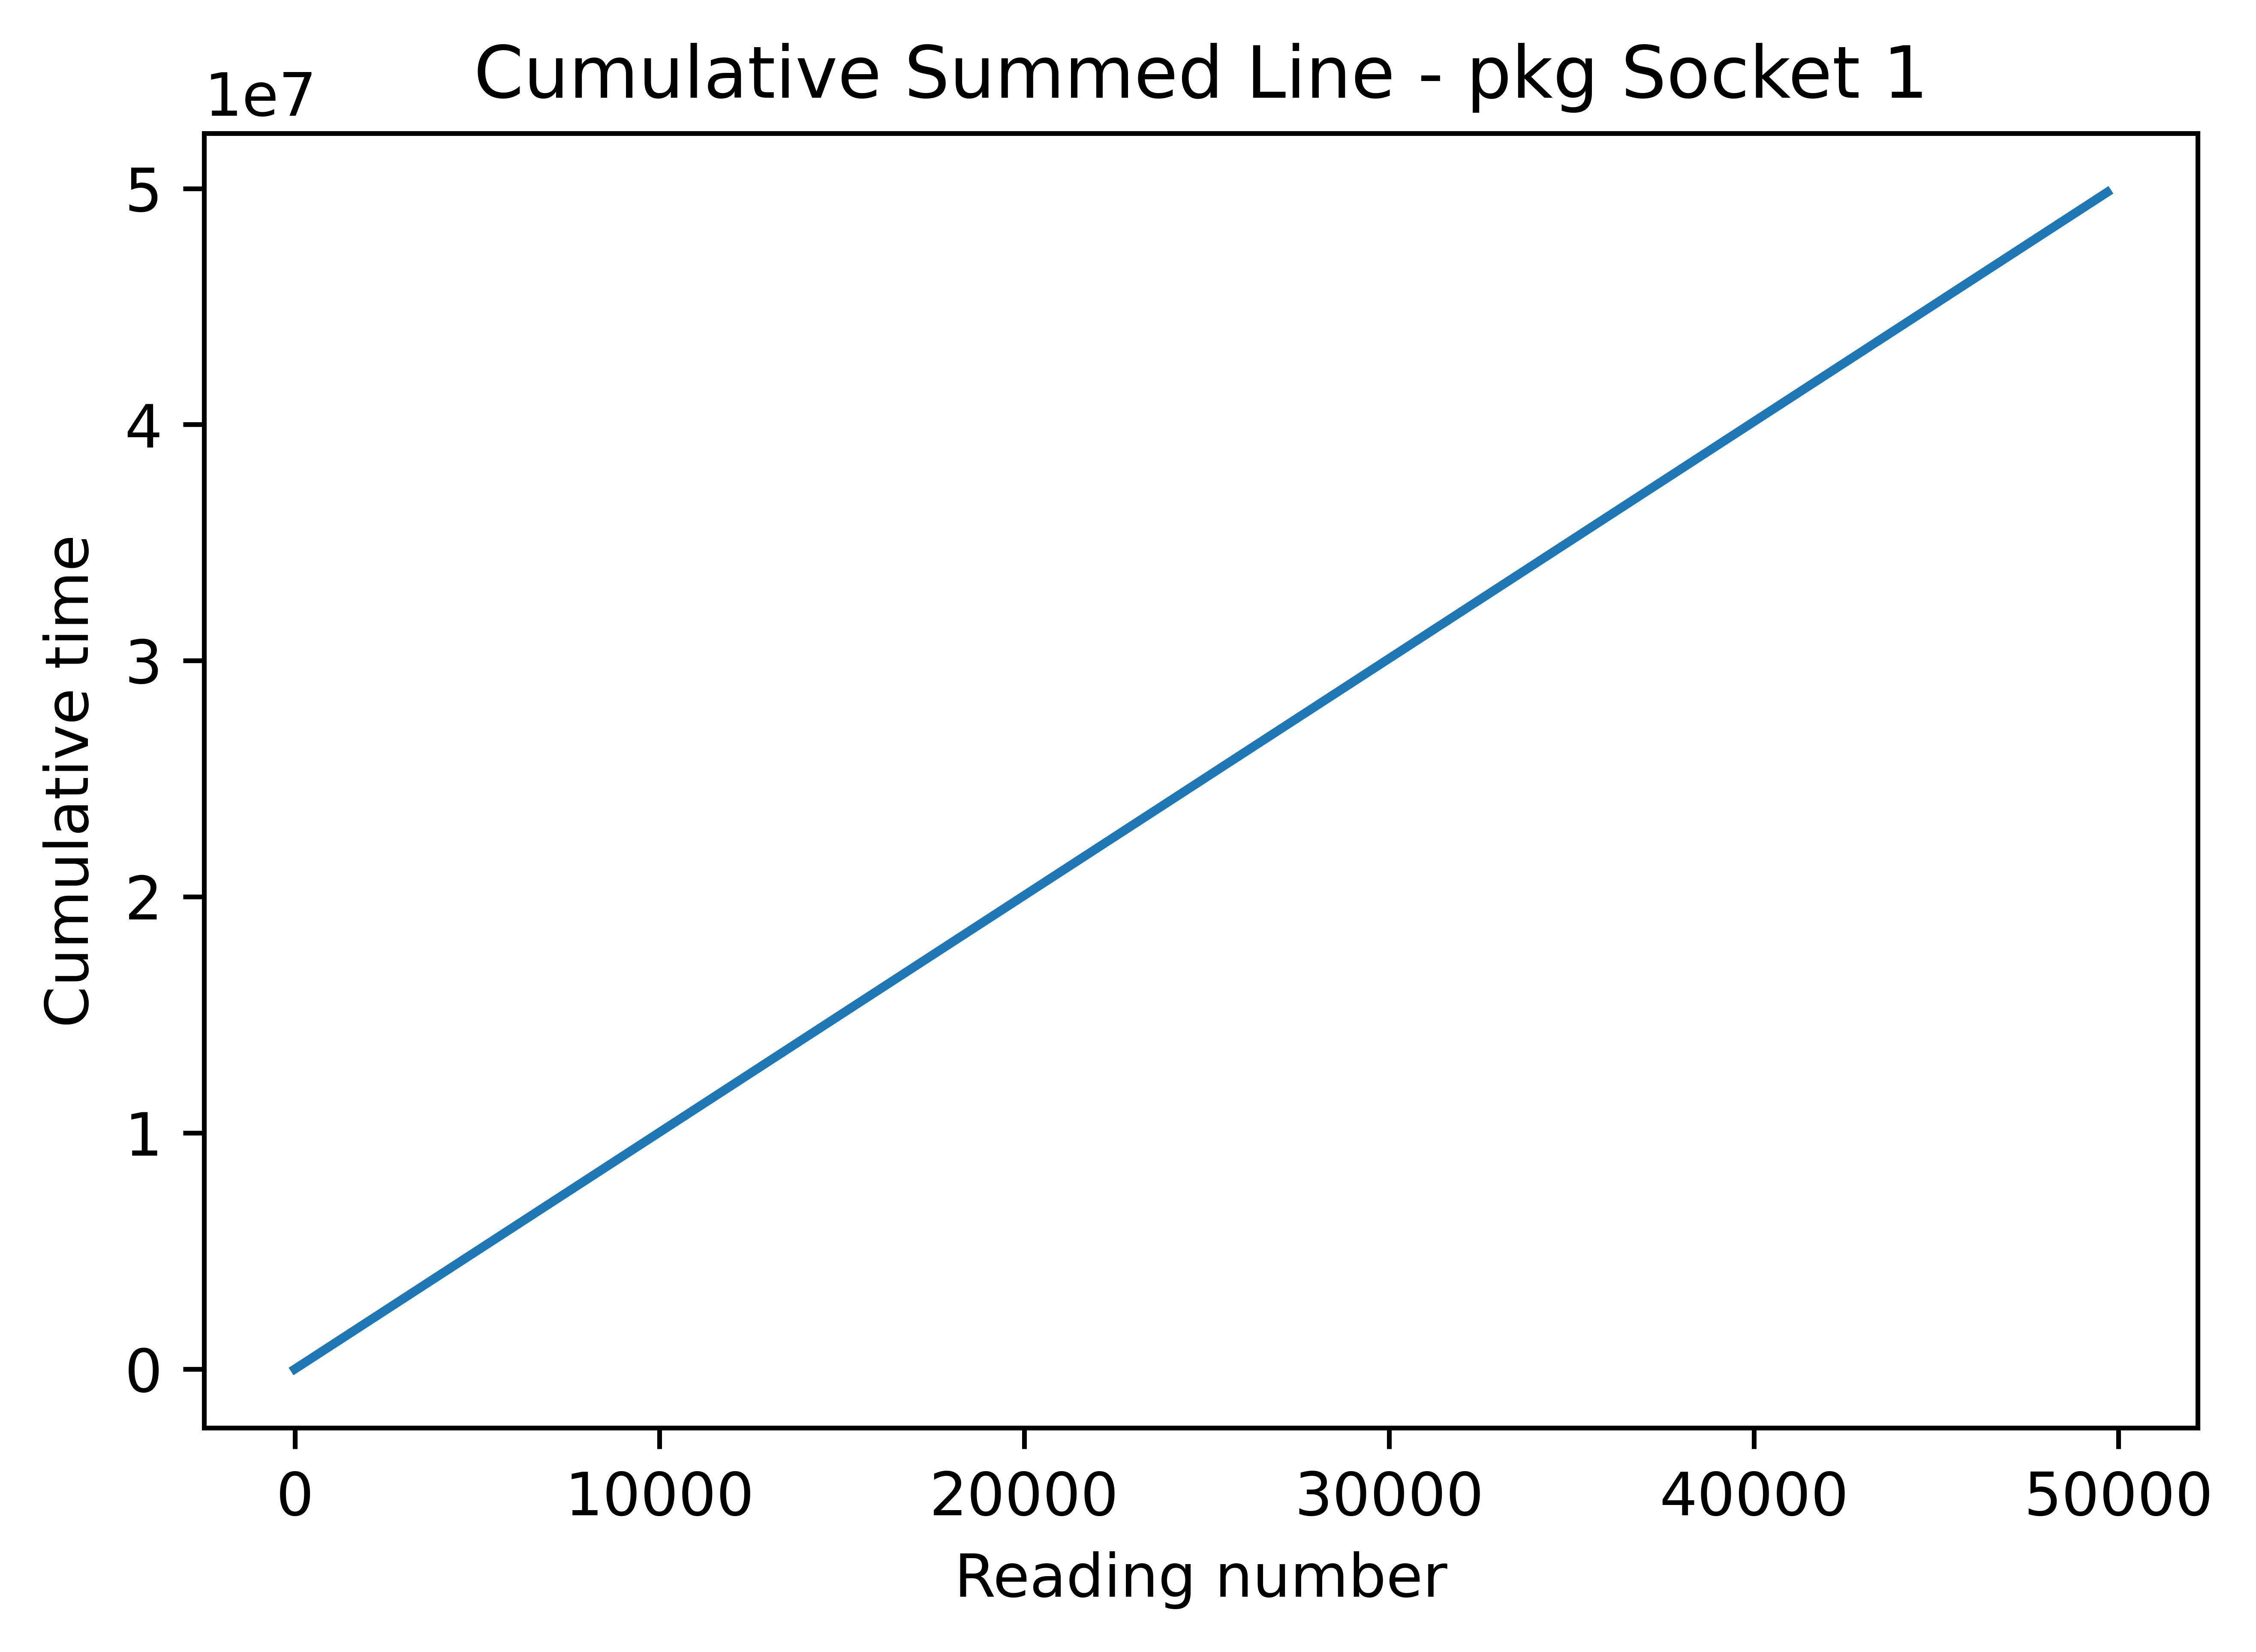
\includegraphics[width=10cm,height=10cm,keepaspectratio]{jmh/msr-update-rate/pkg_Socket_1-cumulative-summed.png}
    \caption{How long it takes for the PKG\_socket2 MSR to update (microseconds)}
    \label{fig:PKG-rapl-counter}
\end{figure}

Dram Socket 0
%\begin{tabular}{lr}
\toprule
{} &   dram_Socket_0_stats \\
ener_diff-vs-num_samples_bw_nonequal & 0.09196352210370197 \\
unique_reading_num-vs-num_samples_bw_nonequal & 0.043276824463455 \\
unique_reading_num-vs-ener_diff & 0.003172218193282899 \\
num_readings & 28367 \\
avg_readings_bw_2_nonequal & 81.62430374391877 \\
s-d_readings_bw_2_nonequal & 884.6362835246799 \\
avg_energy_reading & 0.003991888175985325 \\
s-d_energy_reading & 0.0953152701302277 \\
\bottomrule
\end{tabular}
Dram socket 1
%\begin{tabular}{lr}
\toprule
{} &   dram_Socket_1_stats \\
CC-Energy-Diff-Samples-Between-Non-Equal & -0.020623387258556596 \\
unique_reading_num-vs-num_samples_bw_nonequal & 0.21491816248921825 \\
unique_reading_num-vs-ener_diff & 0.003996556579638411 \\
num_readings & 49240 \\
avg_readings_bw_2_nonequal & 47.180974430837345 \\
s-d_readings_bw_2_nonequal & 6.56195152990962 \\
avg_energy_reading & 0.004011125327484356 \\
s-d_energy_reading & 0.1027373294019606 \\
\bottomrule
\end{tabular}
Pkg Socket 0
%\begin{tabular}{lr}
\toprule
{} &   pkg_Socket_0_stats \\
ener_diff-vs-num_samples_bw_nonequal & -0.06335433066734152 \\
unique_reading_num-vs-num_samples_bw_nonequal & 0.31326217470897305 \\
unique_reading_num-vs-ener_diff & -0.003051859116440657 \\
num_readings & 49699 \\
avg_readings_bw_2_nonequal & 46.73574389311441 \\
s-d_readings_bw_2_nonequal & 4.58756655790207 \\
avg_energy_reading & 0.021698225280695347 \\
s-d_energy_reading & 0.44581372176337347 \\
\bottomrule
\end{tabular}
Pkg Socket 1
%\input{jmh/msr-update-rate/pkg-Socket-1-stats}